% Between 2 and 3 pages
% General project background, research question, and objectives.
% About 5-10 references

\subsection{Background and Motivation}\label{sec:motivation-and-background}

\subsubsection{Location-based Services}\label{sec:location-based-services}

Location-based Services (LBSs) is a large field which has seen an explosion in academic and industry interest~\cite{Junglas2008} since the beginning of the 21st century.
Broadly speaking, it covers information-technology services involved in the collection, analysis and application of any data that tracks the location of either objects, devices or people.
Much of the interest has stemmed from its potential for interdisciplinary use and insight into geographical social trends and tendencies.
It has seen applications in security, health and marketing (mainly for advertising).

Historically, positioning in LBSs has been restricted to use by those who own the infrastructure, namely telecom operators.
~\citeasnoun{Bellavista2008} note the past monopolistic infrastructure-centric nature of both indoor and outdoor localisation and describe this as the shift from operator-centric to user-centric management of LBSs.

As they cover such a wide range of services, LBSs can be grouped by certain characteristics and scopes of usage.
Within the field of localisation, an important divide is made between indoor and outdoor LBSs.
Outdoor LBSs primarily make use of GPS and telecom towers for positioning.
A large example of an outdoor LBS which uses GPS is satellite navigation and social media geotagging which, as of 2013 saw a large usage uptake~\cite{zickuhr2013}.

On the other hand, GPS and telecom tower triangulation is not suitable for indoor positioning.
Even though its possible to receive GPS signal indoors with modern hardware, studies such as \cite{merry2019smartphone} have shown it to be accurate to between 7 and 13 metres outdoors.
This kind of accuracy is only enough to place a device in a building or potentially a large room.
Additionally, GPS elevation is only accurate to between 10 and 20 metres, which is not enough to accurately detect what floor a device is on.
Hence, for better lateral/longitudinal and vertical accuracy, a different localisation technique is required for indoor LBSs.

\subsubsection{Indoor Position Tracking}\label{sec:indoor-position-tracking}

Indoor positioning, or indoor localisation, typically involves tracking the location of people, or groups of people as they move around some premises.
The hardware and software used to achieve this is called an indoor positioning system (IPS), sometimes also referred to as an indoor localisation system (ILS).

IPSs come in many forms and can be broadly split into two groups: computer vision (CV)-based and device-based.
CV-based IPSs have seen increased use recently in line with advancements in state-of-the-art CV object-tracking and facial-recognition methods.
Device-based IPSs typically use wireless technologies such as 802.11 (Wi-Fi)~\cite{ieee1997}, Bluetooth, Bluetooth Low Energy (BLE) and RFID~\cite{S.Shen2020}.
Despite being an exciting technology, a large problem with CV-based IPSs is that they present a much greater privacy risk than device-based IPSs.
This is not only due to the potential for (and incentivised use of) facial recognition, but also the ethical issues with regards to the recording (and storing of recordings) of individuals.

An advantage of 802.11 IPSs is that tracking can be done completely passively.
Almost all modern smartphones have Wi-Fi capability and are constantly sending probe requests to scan for Access Points (APs).
Because of this, their implementation and use of the protocol is all that is required to detect devices.

Received Signal Strength (RSS) is a measure, in decibels, of how strong a signal between two devices are -- these devices are typically a smartphone and a wireless 802.11 AP.
Since RSS is inversely proportional to distance, obtaining the RSS from three APs is enough to triangulate a mobile device to a reasonable degree of accuracy, this is demonstrated in Figure~\ref{fig:triangulation}.
Some IPSs additionally make use of Received Response Time (RRT) and some APs contain additional hardware to calculate Angle of Arrival (AOA), both of which can be used to further increase localisation accuracy.

\begin{figure}[!ht]
    \centering
    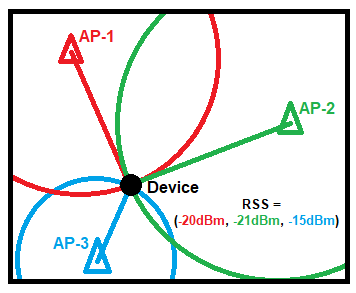
\includegraphics[scale=0.4]{figures/triangulation.png}
    \caption{Triangulation of a mobile device from three APs using RSS.}
    \label{fig:triangulation}
\end{figure}

\subsubsection{MAC Address Randomisation}\label{sec:mac-randomisation}

The operating system of a device is ultimately responsible for implementing the protocols it uses.
As such, there is no way to enforce a device sending its true physical Media Access Control (MAC) address.
This enables the operating system to handle 802.11 communication (including sending probe requests and connecting) with a MAC address of their choice.

Consider the two most widely used operating systems for mobile smartphones: iOS and Android.
Both iOS 8, released in 2014, and Android 6, released in 2015, introduced MAC randomisation in probe requests as the default behaviour.
Since then, both iOS 14, released in 2020, and Android 9, released in 2018, implement full MAC randomisation when connecting to networks.
Whereas the iOS implementation rotates the randomised MAC address every 24 hours, Android retains the same (originally randomised) address per 802.11 SSID\@.
In 2019, Android 10 set this as the default behaviour (as does iOS 14).

While these measures have little practical impact on the user experience when using guest Wi-Fi provided by businesses, it is catastrophic for LBSs which rely on 802.11 probe requests to identify users and their location.
In practice, this means that LBSs are, at best, able to pinpoint the location of a device but not detect its movement over a time period (where MAC randomisation for probe requests is on a fixed timer).
At worst, they are not able to pinpoint a device at all (when MAC addresses are randomised between probe requests).

\subsection{802.11 fingerprinting}\label{sec:wifi-fingerprinting}

Since before the widespread adoption of MAC randomisation, passive 802.11 fingerprinting has been a hot topic for research~\cite{Pang2007}.
In the context of the 802.11 protocol, fingerprinting may either refer to the spatio-temporal identification of individual devices or the pre-processing of specific buildings to calibrate or improve localization success rate of an algorithm.
For the remainder of this paper, assume fingerprinting refers to the former unless otherwise stated.
Additionally, take `MAC de-randomisation' to mean the process of uniquely identifying a device across space and time.

This paper considers two primary forms of fingerprinting techniques for MAC de-randomisation: implicit identifier fingerprinting proposed by~\citeasnoun{Pang2007} and timing attacks proposed by~\citeasnoun{Matte2016} (both of which work on the physical-layer of the OSI model).
A third technique that is considered, which does not involve fingerprinting, works on the link-layer of the OSI model and will be referred to as MAC vendor analysis.
Broadly-speaking, implicit identifier fingerprinting exploits minor differences in manufacturing within the tolerances of mobile devices to uniquely identify them.
Timing attacks use the Inter-frame Arrival Times (IAT) of sets of frames to group them by likelihood of them being sent from the same device.
MAC vendor analysis uses knowledge of how manufacturers assign the lower-order bytes of addresses to devices to infer information about the device.
These are discussed in greater detail as part of Sections~\ref{sec:related-work} and~\ref{sec:solution}.

\subsection{Aims}\label{sec:aims}

The primary objective of this paper is to compare a hybrid implementation consisting of implicit-identifier 802.11 fingerprinting, timing attacks and vendor analysis compared to their individual use.
To assist with this, the paper also aims to produce a Monte Carlo-based location data simulation method to benchmark and test the systems.
Finally, this paper aims to evaluate the hybrid tracking technique when generalised to groups of moving devices.

This research aims to address the following questions:
\begin{enumerate}
    \itemsep-0.5em
    \item What are the differences and similarities between the performance of 802.11 fingerprinting, timing attacks and MAC vendor analysis applied independently compared to them combined into one hybrid method?
    \item How well does this hybrid method generalise to groups of individuals?
    \item How well do these different methods work when applied across the different versions of 802.11?
    \item How can real-world location data be simulated for a controlled testing and evaluation environment?
\end{enumerate}
